\documentclass[12pt]{jarticle}
\usepackage[dvipdfmx]{graphicx}
\title{プログラミング工学・演習課題}
\author{工学部情報工学科 4619072 服部翼}
\begin{document}
\maketitle
\section{バッファオーバフローとは}
まず、「バッファ」というのはコンピュータにおいて出力する速さと入力する速さのズレを補うために、
データを一時的に保持しておくためのメモリ上に確保された領域である。
あらかじめ確保されていたバッファを上回る量のデータが入力された場合、
データが入りきらず隣接する別のメモリに影響を与える可能性がある。
これをバッファオーバフローという。
\section{実例}
ここでC言語を用いてバッファオーバフローの実例を見ていく。\\

\begin{figure}
    \begin{minipage}[t]{0.5\columnwidth}
        \begin{center}
            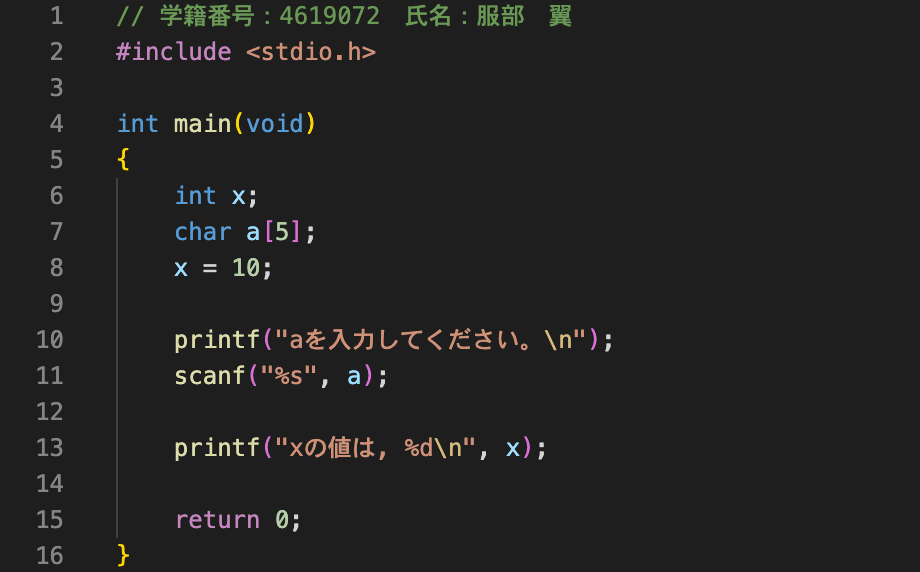
\includegraphics[clip, width=0.9\columnwidth]{SampleA.png}
        \end{center}
        \caption{SampleAのコード}
        \label{fig:left}
    \end{minipage}
    \begin{minipage}[t]{0.5\columnwidth}
        \begin{center}
            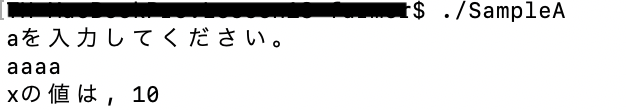
\includegraphics[clip, width=0.9\columnwidth]{A_4.png}
        \end{center}
        \caption{入力例1(a)}
        \label{fig:right}
    \end{minipage}
\end{figure}

図1のコードではサイズ5の文字列型配列aのバッファがすでに確保されており、
また整数型変数xに10が代入されている。

図2のように、配列aに四文字までの文字列を入力するとnull文字も合わせてサイズ5に収まるため、
通常通りxの値は10と表示されている。\\

\begin{figure}[h]
    \begin{center}
        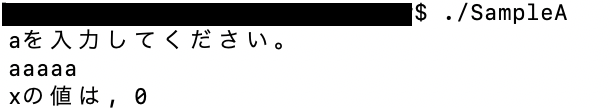
\includegraphics[width=8cm]{A_5.png}
        \caption{入力例1(b)}
        \label{ラベル}
    \end{center}
\end{figure}

次に図3のように、五文字以上の文字列を入力してみるとここでバッファオーバフローが発生し、
xの値を格納していたメモリが不正な値になり、正しく表示されなくなる。\\

\begin{figure}[h]
    \begin{minipage}[t]{0.5\columnwidth}
        \begin{center}
            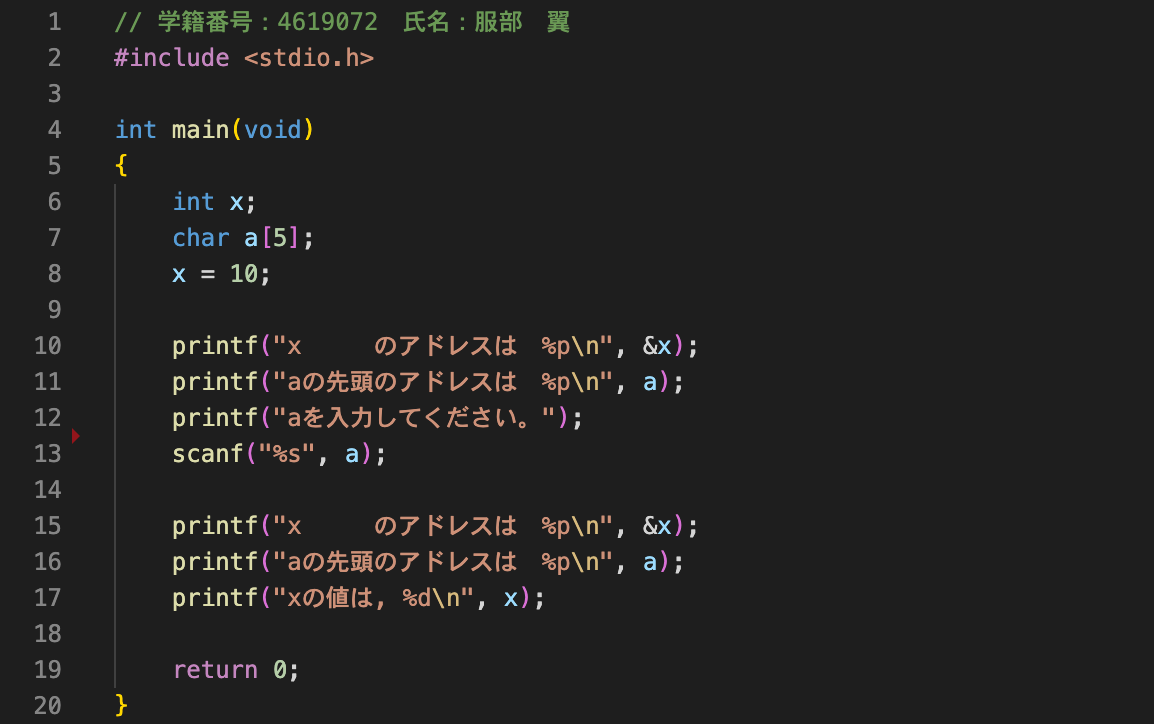
\includegraphics[clip, width=0.9\columnwidth]{SampleB.png}
        \end{center}
        \caption{SampleBのコード}
        \label{fig:left}
    \end{minipage}%
    \begin{minipage}[t]{0.5\columnwidth}
        \begin{center}
            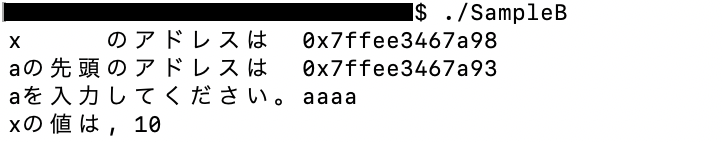
\includegraphics[clip, width=0.9\columnwidth]{B_4.png}
        \end{center}
        \caption{入力例2(a)}
        \label{fig:right}
    \end{minipage}
\end{figure}

図4のコードを実行した結果をみると、xのアドレスは配列aの先頭のアドレスの5byte後ろにあることがわかる。
図5の入力例2(a)ではサイズ1byteの文字(char型)が4つとnull文字を合わせて5byteのデータが入力されており、
あらかじめ確保していたバッファに収まる。\\

\begin{figure}[h]
    \begin{center}
        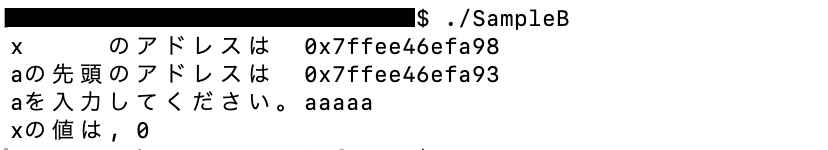
\includegraphics[width=8cm]{B_5.png}
        \caption{入力例2(b)}
        \label{ラベル}
    \end{center}
\end{figure}

今度は図6の入力例2(b)のように5byteを超えるデータを入力すると配列aのバッファを超えてしまい、
後ろにあるxのメモリに影響を及ぼしてしまうことがわかる。\\

以上のような仕組みでバッファオーバフローが発生する。
これは非常に危険な脆弱性となるため、コードを書くときには入力データを厳密にチェックしたり、
セキュリティ上で危険な関数などは使わないようにすることが重要である。
\end{document}